\subsection{Operation Model for oeCreateSystemAndEnvironment}

\label{OM-oeCreateSystemAndEnvironment}


The \msrcode{oeCreateSystemAndEnvironment} operation has the following properties:

	\begin{operationmodel}
	\addheading{Operation}
	\adddoublerow{oeCreateSystemAndEnvironment}{sent to request the initialization of the system's class instances and the environment actors instances.}

	\addrowheading{Parameters}
	\addnumbereddoublerow{}{AqtyComCompanies: ptInteger}{the quantity of communication companies to create in the environment} 

	\addrowheading{Return type}
	\addsinglerow{ptBoolean}

	\addrowheading{Pre-Condition (protocol)}
	\addnumberedsinglerow{PreP}{ none}
		
	\addrowheading{Pre-Condition (functional)}
	\addnumberedsinglerow{PreF}{ none }

	\addrowheading{Post-Condition (functional)}
	\addnumberedsinglerow{PostF}{ the ctState instance is initialized with the integer 1 for the crisis and alert counters used for their identifications, a value for the clock corresponding to a default inital time (i.e. January 1st, 1970) the crisis reminder period is set to 300 seconds, the maximum crisis reminder period is fixed to 1200 seconds (i.e. 20 minutes), an initial value for the automatic reminder period equal to the current date and time and the system is considered in a started state.
	
	{\bf Those predicates must be satisfied first since all the other depend on the existence of a ctState instance !}}
	\addnumberedsinglerow{PostF}{the \msrcode{actMsrCreator} actor instance is initiated (remember that since the \msrcode{oeCreateSystemAndEnvironment} is a special event it role is to make consistent the post state thus creating the actor and its interfaces is required even though the sending of this message logically would need the actor and its interfaces to already exist ...).}
	\addnumberedsinglerow{PostF}{the environment for communication company actors, in the post state, is made of \msrcode{AqtyComCompanies} instances allowing for receiving and sending messages to humans.}
	\addnumberedsinglerow{PostF}{the environment for administrator actors, in the post state, is made of one instance.}
	\addnumberedsinglerow{PostF}{the environment for activator actors, in the post state, is made of one instance allowing for automatic message sending based on current system's and environment state'.}
	\addnumberedsinglerow{PostF}{the set of ctAdministrator instances at post is made of one instance initialized with 'icrashadmin' (resp. '7WXC1359') for login (resp. password) values.}
	\addnumberedsinglerow{PostF}{the association between ctAdministrator and actAdministrator is made of one couple made of the conjointly specified instances.}

	\addrowheading{Post-Condition (protocol)}
	\addnumberedsinglerow{PostP}{ none is given since the only protocol variable to be modified in the post state is the one initialized with the ctState instance (i.e. vpStarted).}
	\end{operationmodel}



	% ------------------------------------------
	% MCL Listing
	% ------------------------------------------
	\vspace{1cm}
	The listing~\ref{OM-actMsrCreator-oeCreateSystemAndEnvironment-MCL-LST} provides the \msrmessir (MCL-oriented) specification of the operation.
	
	\scriptsize
	\vspace{0.5cm}
	\begin{lstlisting}[style=MessirStyle,firstnumber=auto,captionpos=b,caption={\msrmessir (MCL-oriented) specification of the operation \emph{oeCreateSystemAndEnvironment}.},label=OM-actMsrCreator-oeCreateSystemAndEnvironment-MCL-LST]

	/* Pre Protocol:*/ 
	preP{true}
	
	/* Pre Functional:*/
	preF{true}
	
	/* Post Functional:*/ 
	postF{let TheSystem: ctState in
	  let AactMsrCreator: actMsrCreator in
	  let AactAdministrator: actAdministrator in
	  let AnextValueForAlertID: dtInteger in
	  let AnextValueForCrisisID: dtInteger in
	  let Aclock: dtDateAndTime in
	  let AcrisisReminderPeriod: dtSecond in
	  let AmaxCrisisReminderPeriod: dtSecond in
	  let AvpStarted: ptBoolean in
	
	  /* PostF01 -- MUST ALWAYS BE MADE FIRST -- */ 
	  AnextValueForAlertID.value.eq(1)
	  and AnextValueForCrisisID.value.eq(1)
	  and Aclock.date.year.value = 1970 
	  and Aclock.date.month.value = 01
	  and Aclock.date.day.value = 01
	  and Aclock.time.hour.value = 00
	  and Aclock.time.minute.value = 00
	  and Aclock.time.second.value = 00
	
	  and AcrisisReminderPeriod.value.eq(300)
	  and AmaxCrisisReminderPeriod.value.eq(1200)
	  and AvpStarted = true
	  and TheSystem.init(AnextValueForAlertID,
	                     AnextValueForCrisisID,
	                     Aclock,
	                     AcrisisReminderPeriod,
	                     AmaxCrisisReminderPeriod,
	                     Aclock,
	                     AvpStarted
	                    )
	  /* PostF02*/ 
	  and AactMsrCreator.init()
	  /* PostF03 */ 
	  and let AactComCompanyCol: Bag(actComCompany) in
	  AactComCompanyCol->size() = AqtyComCompanies
	  AactComCompanyCol-> forAll(init())
	 /* PostF04*/ 
	  and AactAdministrator.init()
	  /* PostF05*/ 
	  and let AactActivator:actActivator in
	  AactActivator.init()
	/* PostF06 */ 
	  and let ActAdministrator:ctAdministrator in
	      let AdtLogin:dtLogin in
	      let AdtPassword:dtPassword in
	      AdtLogin.value.eq('icrashadmin')
	      and AdtPassword.value.eq('7WXC1359')
	      and ActAdministrator.init(AdtLogin,AdtPassword)
	 /* PostF07*/ 
	  and ActAdministrator@post.rnactAuthenticated = AactAdministrator}
	
	/* Post Protocol:*/ 
	postP{ true}
	
	\end{lstlisting}
	\normalsize 
	
	
	
	





Figure \ref{fig:lu.uni.lassy.excalibur.examples.icrash-OM-scopeView-operation-scope-outactMsrCreator-oeCreateSystemAndEnvironment}
shows all the concept model elements in the scope of the oeCreateSystemAndEnvironment operation

\begin{figure}[htbp]
\begin{center}

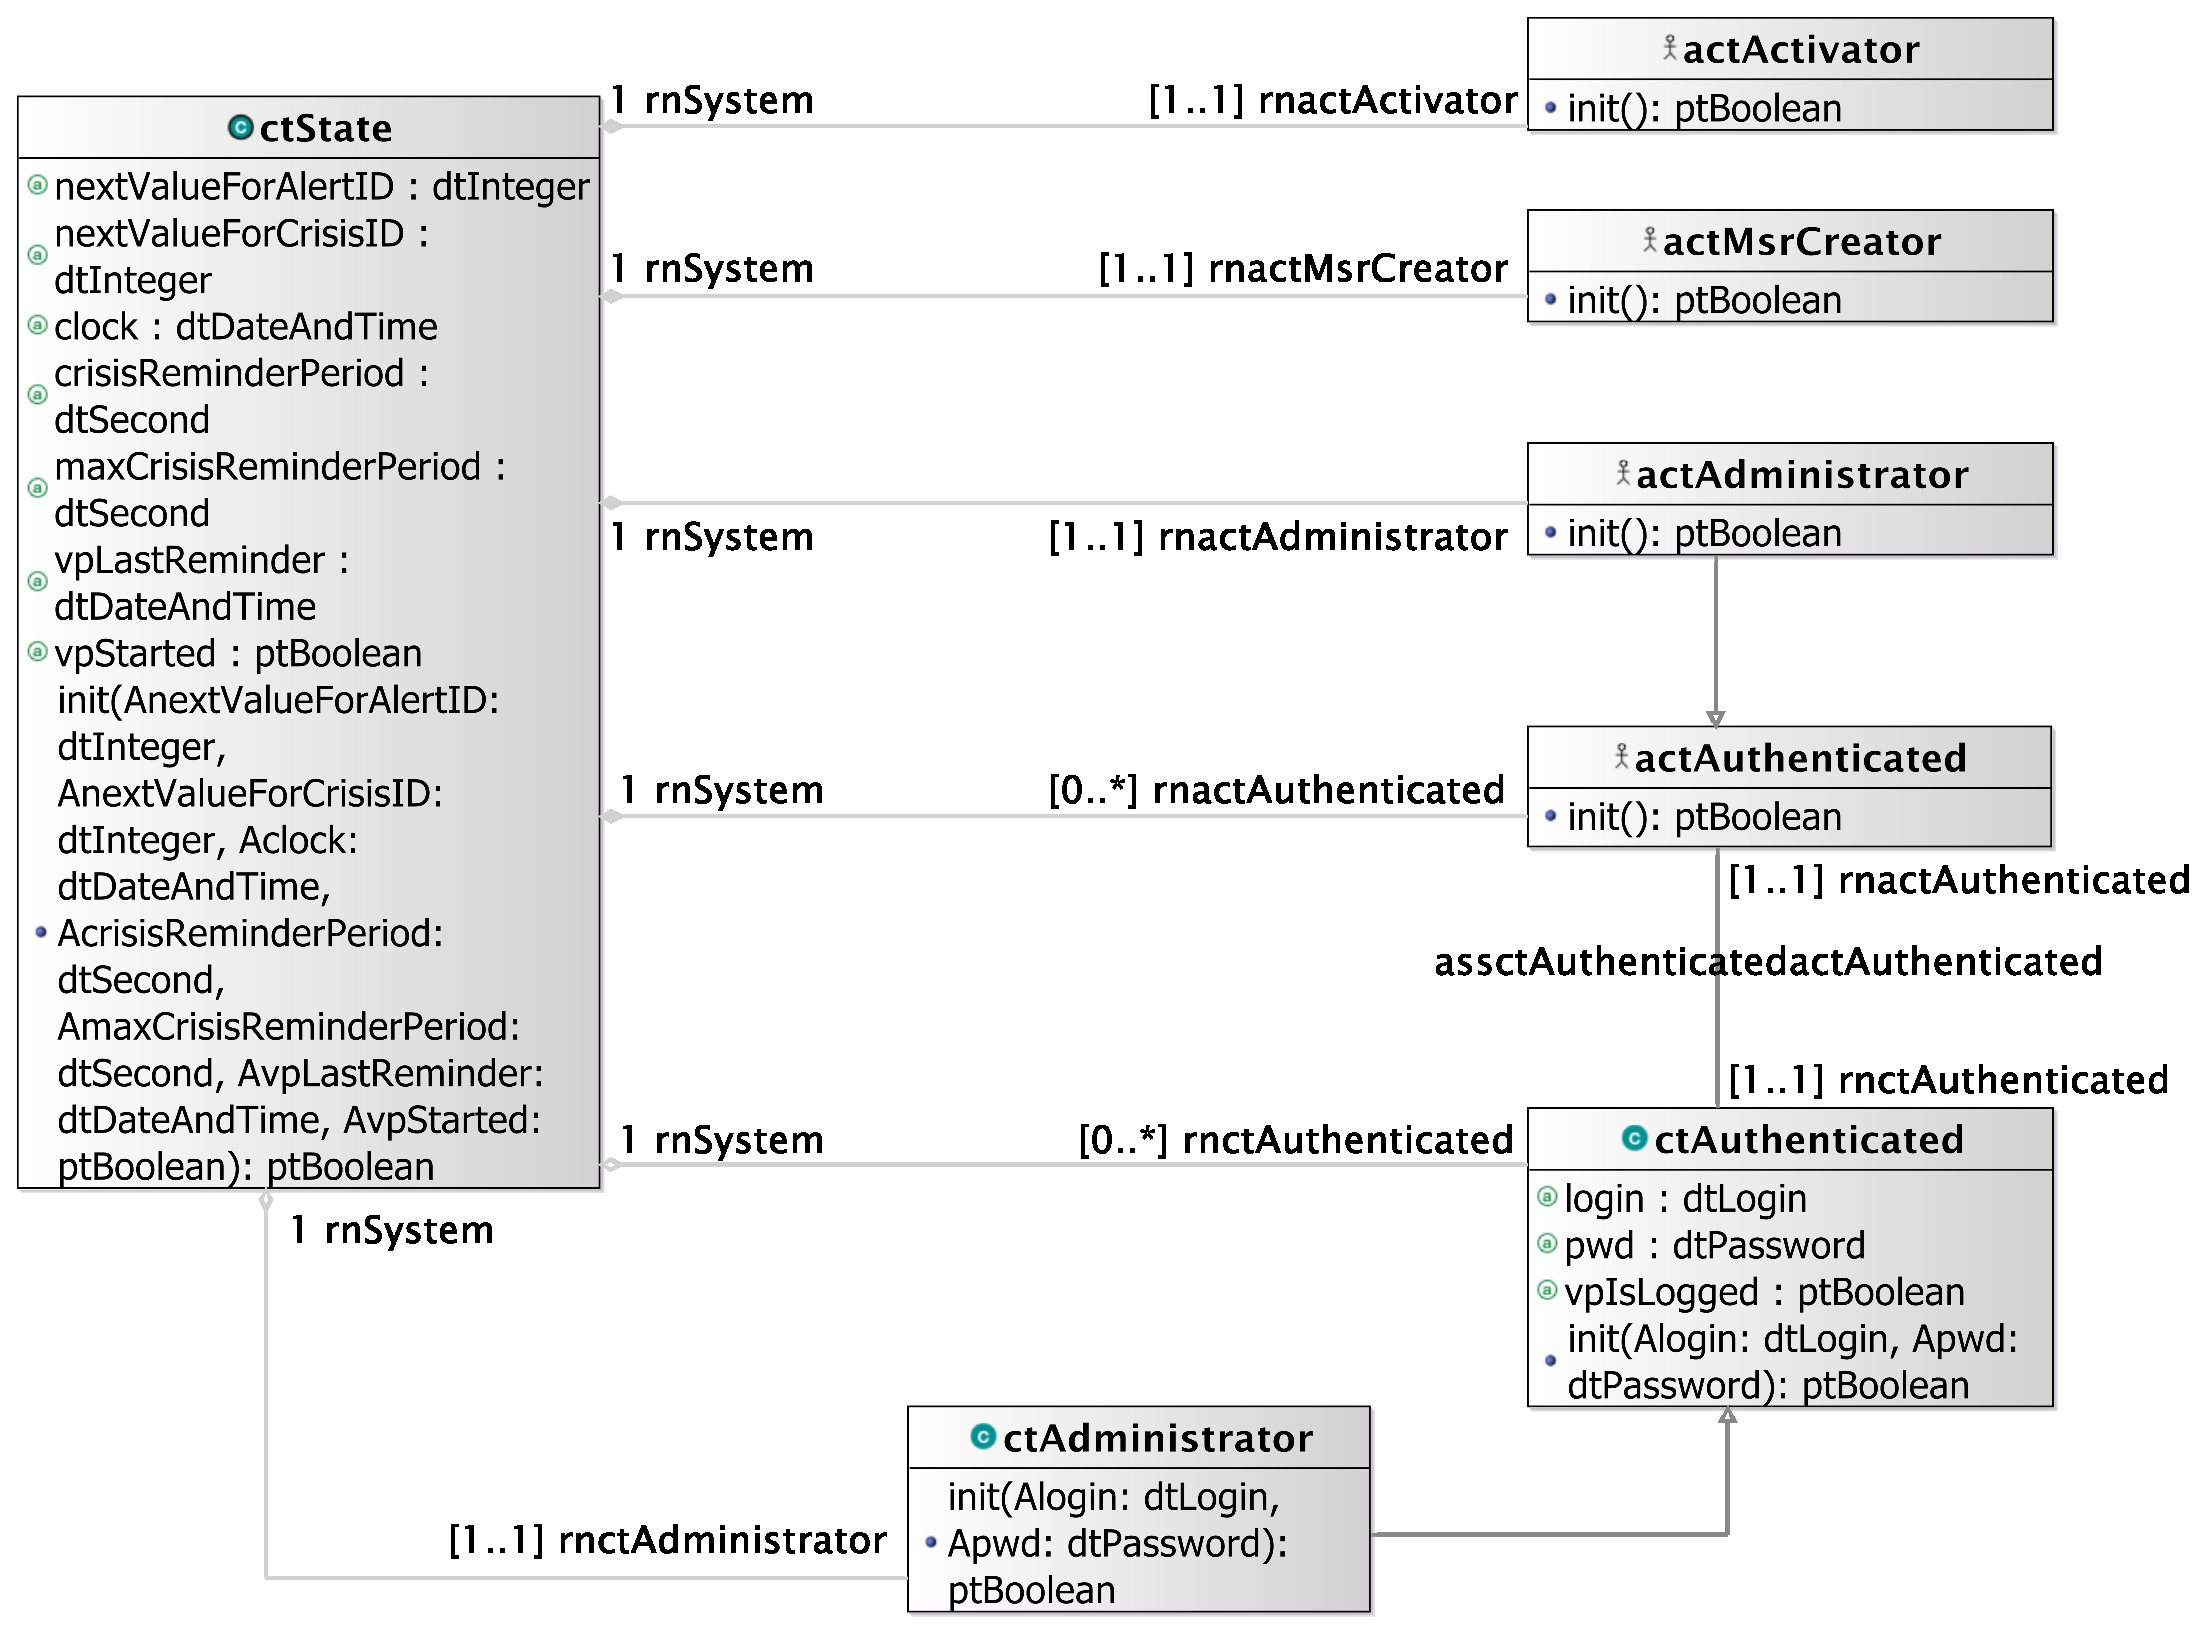
\includegraphics[
angle=0
,width=1.0\textwidth
]{./images-report-gen/operation-model/operation-scope-outactMsrCreator-oeCreateSystemAndEnvironment.eps}
\end{center}
\caption[lu.uni.lassy.excalibur.examples.icrash Operation Scope: operation-scope-outactMsrCreator-oeCreateSystemAndEnvironment]{oeCreateSystemAndEnvironment operation scope
}
\label{fig:lu.uni.lassy.excalibur.examples.icrash-OM-scopeView-operation-scope-outactMsrCreator-oeCreateSystemAndEnvironment}
\end{figure}
\vspace{0.5cm}

